\documentclass[UTF8,zihao=-4]{ctexbeamer}
\usepackage{multimedia}
\usepackage{hyperref}

%\usetheme{AnnArbor}
%\usetheme{Antibes}
%\usetheme{Marburg}
%\usetheme{boxes}
%\usetheme{Szeged}
%\usetheme{Goettingen}
%\usetheme{Szeged}	
\usetheme{Madrid}
%\useoutertheme{miniframes}

\usecolortheme{orchid}
\title{数控编程概术}
\author{高星}
\institute{湖南潇湘技师学院~湖南九嶷职院}
\date{2018.09.14}
\begin{document}
\begin{frame}[plain]
		\maketitle
\end{frame}

\begin{frame}
\begin{columns}
\column[t]{0.3\textwidth}
\column[t]{0.7\textwidth}
\tableofcontents[hideallsubsections]
\end{columns}
\end{frame}

\section{制造自动化技术的发展}
\subsection{教学目标}
\begin{frame}{教学目标}
\begin{columns}
	\column{.2\textwidth}
	\column{.8\textwidth}
	\begin{enumerate}
	\item 了解制造自动化技术的发展;
	\item 掌握数控技术的基本概念;
	\item 了解数控机床的组成与工作过程;
	\item 了解数控机床的种类;
	\item 掌握数控机床的坐标系。
\end{enumerate}
\end{columns}
\end{frame}

\subsection{制造自动化技术的发展}
\begin{frame}[<+->]{制造自动化技术的发展}
%\begin{columns}
%	\column{.1\textwidth}
%	\column{.9\textwidth}
	\begin{itemize}
		\item 人工控制——手动操作
		\item 刚性自动化——在20世纪40~50年代已相当成熟。应用传统的机械设计与制造工艺方法,采用专用机床和组合机床、自动单机或自动化生产线进行大批量生产。其特征是高生产率和刚性结构,很难实现生产产品的改变。引入的新技术包括继电器程序控制、组合机床等。 
		\item 数控加工——包括数控(NC)和计算机数控(CNC)。特点是柔性好、加工质量高,适应于多品种、中小批量(包括单件产品)的生产。引入的新技术包括数控技术、计算机编程技术等。
	\end{itemize}
%\end{columns}
\end{frame}

\begin{frame}[<+->]{制造自动化技术的发展}
%\begin{columns}
%	\column{.1\textwidth}
%	\column{.9\textwidth}
\begin{itemize}
	\item 柔性制造——其特征强调制造过程的柔性和高效率,适应于多品种、中小批量的生产。涉及的技术包括成组技术(GT)、计算机直接数控和分布式数控(DNC)、柔性制造单元(FMC)、柔性制造系统(FMS)、柔性加工线(FML)、离散系统理论和方法、仿真技术、车间计划与控制、制造过程监控技术、计算机控制与通信网络等。
	
\end{itemize}
%\end{columns}
\end{frame}

\begin{frame}[<+->]{制造自动化技术的发展}
%\begin{columns}
%	\column{.1\textwidth}
%	\column{.9\textwidth}
\begin{itemize}	
	\item 计算机集成制造系统(CIMS)——其特征是强调全过程的系统性和集成性,以解决现代企业生存与竞争的 TQCS (Time-提供产品的时间,Quality-产品的质量,Cost-产品的成本,Service-产品的服务)问题。CIMS涉及的学科非常广泛,包括现代制造技术、管理技术、计算机技术、信息技术、自动化技术和系统工程等。
	\item 新的制造自动化模式——如智能制造、敏捷制造、虚拟制造、网络制造、全球制造、绿色制造等。
	\item 工业4.0,中国制造2025等(智能化、物联网、信息化、大数据)。
\end{itemize}
%\end{columns}
\end{frame}

\section{数控技术的基本概念}

\begin{frame}{数控技术的基本概念}
\begin{columns}
	\column{.1\textwidth}
	\column{.8\textwidth}
	\begin{block}{\centering 数控技术}
数控(Numerical Control)技术是用数字化的信息对某一对象进行控制的技术。
控制对象可以是位移、角度、速度等机械量,也可以是温度、压力流量、颜色等物理量,这些量的大小不仅是可以测量的,而且可以经A/D或D/A转换,用数字信号来表示。数控技术是近代发展起来的一种自动控制技术,是机械加工现代化的重要基础与关键技术。
	\end{block}
	\column{.1\textwidth}
\end{columns}
\end{frame}

\begin{frame}{数控技术的基本概念}
\begin{columns}
	\column{.1\textwidth}
	\column{.8\textwidth}
	\begin{block}{\centering 数控加工}
		数控加工是指采用数字信息对零件加工过程进行定义,并控制机床进行自动运行的一种自动化加工方法。
	\end{block}
数控加工是20世纪40年代后期为适应加工复杂外形零件而发展起来的一种自动化技术。1947年,美国帕森斯(Parsons)公司为了精确地制作直升机机翼、浆叶和飞机框架,提出了用数字信息来控制机床自动加工外复杂零件的设想。1949年美国空军为了能在短时间内制造出经常变更设计的火箭零件,与帕森斯公司和麻省理工学院(MIT)伺服机构研究所合作,于1952年研制成功世界上第一台数控机床——三坐标立式铣床,可控制铣刀进行连续空间曲面的加工,揭开了,数控加工技术的序幕。
	\column{.1\textwidth}
\end{columns}
\end{frame}

\begin{frame}{数控技术的基本概念}
\begin{columns}
	\column{.1\textwidth}
	\column{.8\textwidth}
	\begin{block}{\centering 数控机床}
		数控机床就是采用了数控技术的机床。
	
	\end{block}
		数控机床将零件加工过程所需的各种操作和步骤以及刀具与工件之间的相对位移量都用数字化的代码来表示,由编程人员编制成规定的加工程序,通过输入介质(磁盘等)送入计算机控制系统,由计算机对输入的信息进行处理与运算,发出各种指令来控制机床的运动,使机床自动地加工出所需要的零件。
	
	特点有:高精度、高柔性、高效率、减轻工人的劳动强度,改善了劳动条件,有良好的经济效益,有利于生产的管理和现代化
	\column{.1\textwidth}
\end{columns}
\end{frame}

\begin{frame}{数控技术的基本概念}
\begin{columns}
	\column{.1\textwidth}
	\column{.8\textwidth}
	\begin{block}{\centering 数控编程}
		数控编程(NC Programming)就是生成用数控机床进行零件加工数控程序的过程。。
		
	\end{block}
数控程序  是由一系列程序段组成,把零件的加工过程、切削用量、位移数据以及各种辅助操作,按机床的操作和运动顺序,用机床规定的指令及程序格式排列而成的一个有序指令集。如 N10 G00 X200.0 Y-39.0 M03 。
	\column{.1\textwidth}
\end{columns}
\end{frame}


\section{数控机床的组成与工作过程}

\begin{frame}{各种各样的数控机床}
\begin{columns}
	\column{.3\textwidth}
	数控车床是一种用于完成车削加工的数控机床。
	
	\column{.7\textwidth}
    \begin{figure}
    	\centering
    	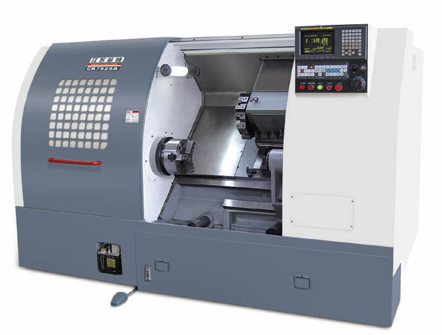
\includegraphics[width= \linewidth]{image/1-1}
%    	\caption{}
    	\label{fig:1-1}
    \end{figure}
\end{columns}
\end{frame}

\begin{frame}{各种各样的数控机床}
\begin{columns}
	\column{.3\textwidth}
	用于完成铣削加工或镗削加工的数控机床。
	
	\column{.7\textwidth}
	\begin{figure}
		\centering
		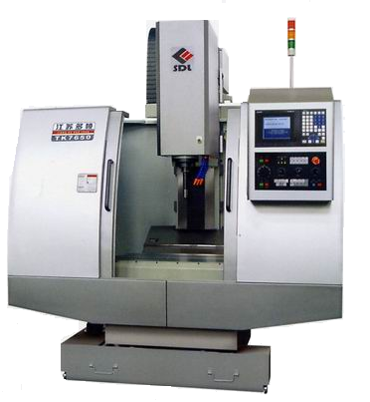
\includegraphics[width= 0.8\linewidth]{image/1-2}
		%    	\caption{}
		\label{fig:1-2}
	\end{figure}
\end{columns}
\end{frame}

\begin{frame}{各种各样的数控机床}
\begin{columns}
	\column{.3\textwidth}
	加工中心是指带有刀库和刀具自动交换装置的数控机床。通常所说的加工中心是指带有刀库和刀具自动交换装置的数控铣床。
	
	\column{.7\textwidth}
	\begin{figure}
		\centering
		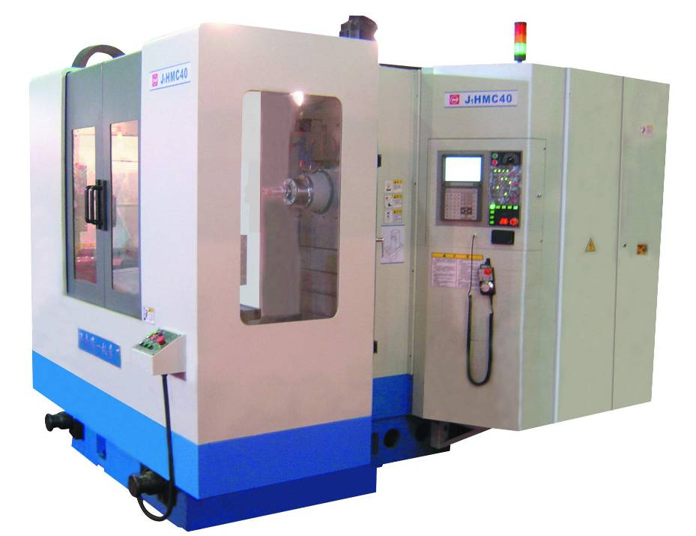
\includegraphics[width= 0.8\linewidth]{image/1-3}
		%    	\caption{}
		\label{fig:1-3}
	\end{figure}
\end{columns}
\end{frame}

\begin{frame}{各种各样的数控机床}
\begin{columns}
	\column{.3\textwidth}
数控钻床是一种采用点位控制系统的数控机床,即控制刀具从一点到另一点的位置,而不控制刀具移动轨迹。
	
	\column{.7\textwidth}
	\begin{figure}
		\centering
		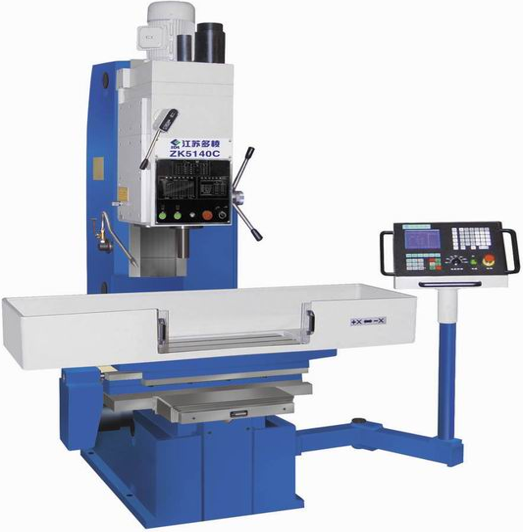
\includegraphics[width= 0.8\linewidth]{image/1-4}
		%    	\caption{}
		\label{fig:1-4}
	\end{figure}
\end{columns}
\end{frame}

\begin{frame}{各种各样的数控机床}
\begin{columns}
	\column{.3\textwidth}
	数控电火花机床是一种特种加工机床,它利用两个不同极性的电极在绝缘液体中产生的电蚀现象去除材料而完成加工。
	
	\column{.7\textwidth}
	\begin{figure}
		\centering
		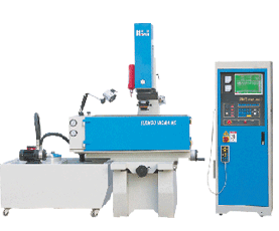
\includegraphics[width= 0.8\linewidth]{image/1-5}
		%    	\caption{}
		\label{fig:1-5}
	\end{figure}
\end{columns}
\end{frame}

\begin{frame}{各种各样的数控机床}
\begin{columns}
	\column{.3\textwidth}
	数控线切割机床其工作原理与电火花成形机床相同,但其电极是电极丝和工件。 
	
	\column{.7\textwidth}
	\begin{figure}
		\centering
		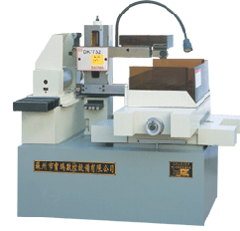
\includegraphics[width= 0.8\linewidth]{image/1-6}
		%    	\caption{}
		\label{fig:1-6}
	\end{figure}
\end{columns}
\end{frame}

\begin{frame}{各种各样的数控机床}
\begin{columns}
	\column{.5\textwidth}
	\begin{figure}
	\centering
	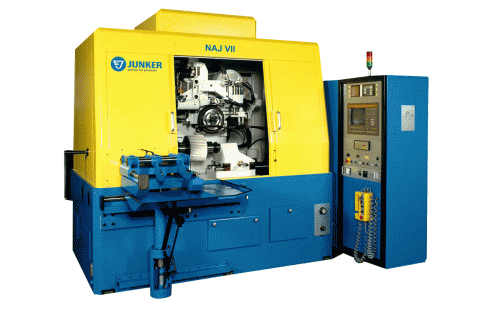
\includegraphics[width= 0.8\linewidth]{image/1-7}
	%    	\caption{}
	\label{fig:1-7}
\end{figure}
	\column{.5\textwidth}
	\begin{figure}
		\centering
		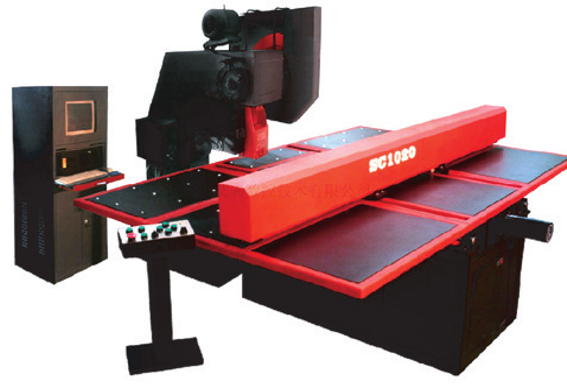
\includegraphics[width= 0.8\linewidth]{image/1-8}
		%    	\caption{}
		\label{fig:1-8}
	\end{figure}
\end{columns}
\end{frame}

\begin{frame}{数控铣床/加工中心的组成}
\begin{columns}
	\column{.3\textwidth}
	\begin{figure}
	\begin{enumerate}	
		\item 工作台 
		\item 刀库 
		\item 换刀装置 
		\item 电动机 
		\item 主轴 
		\item 导轨 
		\item 床身 
		\item 数控系统
	\end{enumerate}
	\end{figure}
	\column{.7\textwidth}
	\begin{figure}
		\centering
		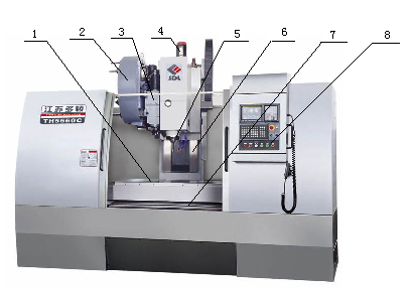
\includegraphics[width= 0.8\linewidth]{image/1-9}
		%    	\caption{}
		\label{fig:1-9}
	\end{figure}
\end{columns}
\end{frame}

\begin{frame}{数控铣床/加工中心的组成}
\begin{columns}
	\column{.3\textwidth}
机床本体部分主要由床身、工作台、立柱、主轴部件等组成。 
	\column{.7\textwidth}
	\begin{figure}
		\centering
		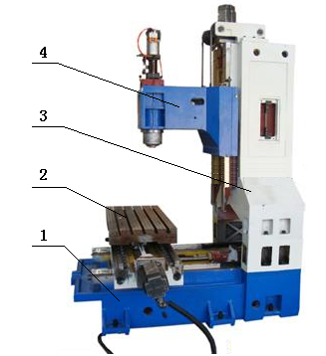
\includegraphics[width= 0.8\linewidth]{image/1-10}
		%    	\caption{}
		\label{fig:1-10}
	\end{figure}
\end{columns}
\end{frame}

\begin{frame}{数控铣床/加工中心的组成}
\begin{columns}
	\column{.3\textwidth}
	数控装置主要由数控系统、伺服驱动装置和伺服电动机组成 。 
	\column{.7\textwidth}
	\begin{figure}
		\centering
		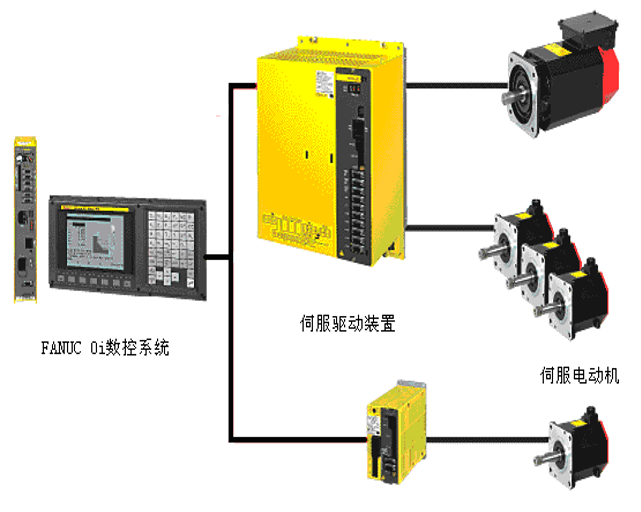
\includegraphics[width= 0.8\linewidth]{image/1-11}
		%    	\caption{}
		\label{fig:1-11}
	\end{figure}
\end{columns}
\end{frame}

\begin{frame}{数控铣床/加工中心的组成}
\begin{columns}
	\column{.3\textwidth}
	数控装置主要由数控系统、伺服驱动装置和伺服电动机组成 。 
	\column{.7\textwidth}
	\begin{figure}
		\centering
		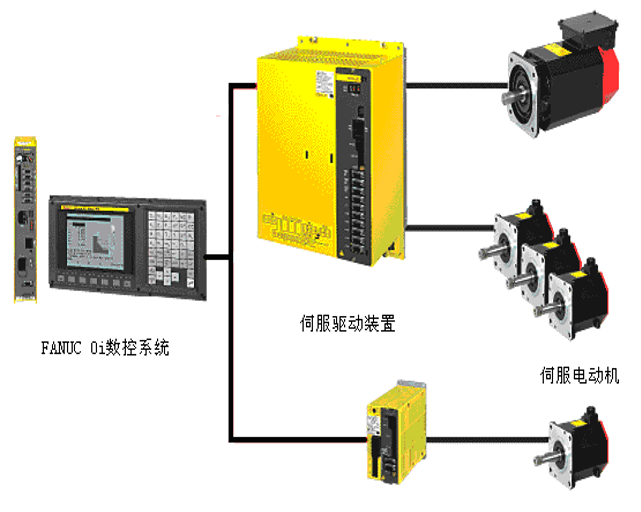
\includegraphics[width= 0.8\linewidth]{image/1-11}
		%    	\caption{}
		\label{fig:1-12}
	\end{figure}
\end{columns}
\end{frame}

\begin{frame}{数控铣床/加工中心的组成}
\begin{columns}
	\column{.2\textwidth}
	刀库和换刀装置  。 
	\column{.8\textwidth}
	\begin{figure}
		\centering
		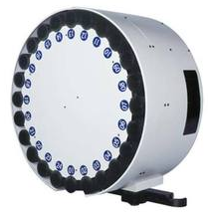
\includegraphics[width= 0.5\linewidth]{image/1-12}
		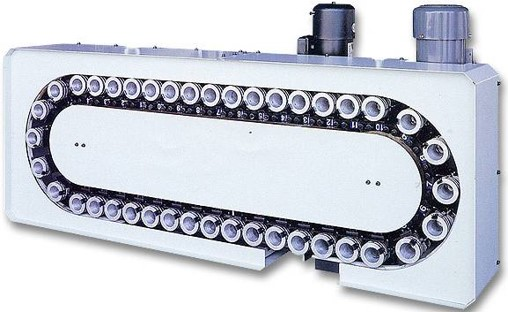
\includegraphics[width= 0.5\linewidth]{image/1-13}
		%    	\caption{}
		\label{fig:1-13}
	\end{figure}

\end{columns}
\end{frame}

\begin{frame}{数控铣床/加工中心的组成}
	加工中心常用的辅助装置有气动装置、润滑装置、冷却装置、排屑装置和防护装置等。  
\begin{columns}
	\column{.25\textwidth}
	\begin{figure}
	\centering
	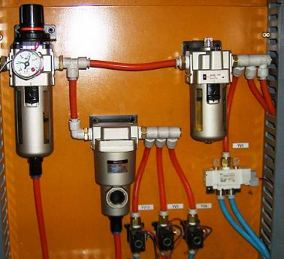
\includegraphics[width= \linewidth]{image/1-14}
	%    	\caption{}
	\label{fig:1-14}
	\end{figure}
	\column{.25\textwidth}
	\begin{figure}
		\centering
		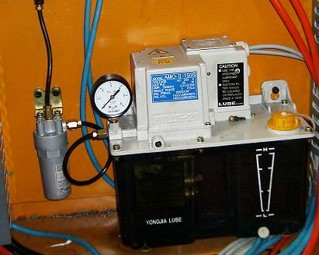
\includegraphics[width= \linewidth]{image/1-15}
		%    	\caption{}
		\label{fig:1-15}
	\end{figure}
	\column{.25\textwidth}
	\begin{figure}
	\centering
	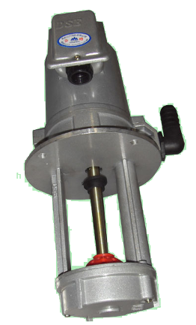
\includegraphics[width= \linewidth]{image/1-16}
	%    	\caption{}
	\label{fig:1-16}
\end{figure}
	\column{.25\textwidth}
	\begin{figure}
	\centering
	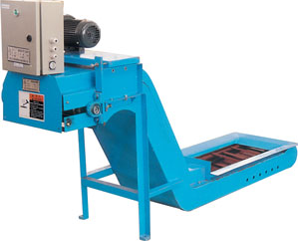
\includegraphics[width= \linewidth]{image/1-17}
	%    	\caption{}
	\label{fig:1-17}
\end{figure}	
\end{columns}
\end{frame}


\begin{frame}{数控铣床/加工中心的组成}
\centering FANUC数控系统由日本富士通公司研制开发。

	\begin{figure}
		\centering
		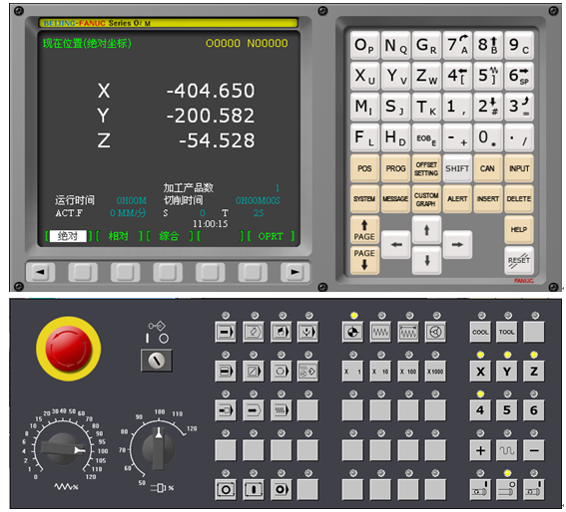
\includegraphics[width= 0.5\linewidth]{image/1-18}
		%    	\caption{}
		\label{fig:1-18}
	\end{figure}
	
\end{frame}

\begin{frame}{数控铣床/加工中心的组成}
\centering SIEMENS数控系统由德国西门子公司研制开发。

\begin{figure}
	\centering
	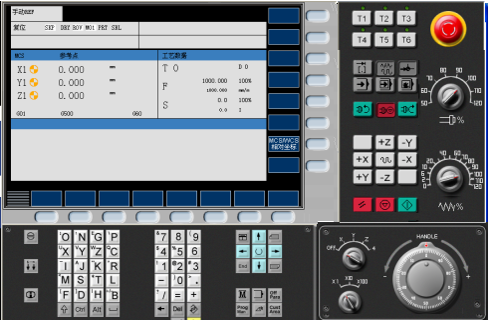
\includegraphics[width= 0.5\linewidth]{image/1-19}
	%    	\caption{}
	\label{fig:1-19}
\end{figure}

\end{frame}

\begin{frame}{数控铣床/加工中心的组成}
\centering 目前,常用于铣床的国产数控系统有北京凯恩地数控系统、华中数控系统、北京航天数控系统等。 

\begin{figure}
	\centering
	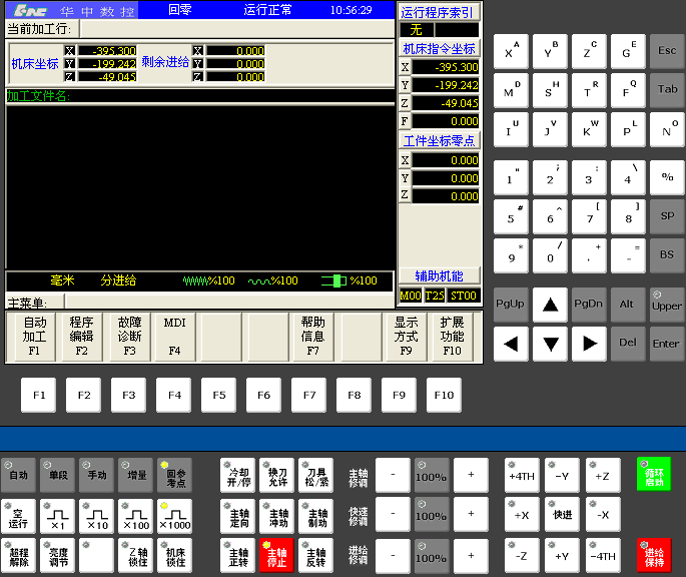
\includegraphics[width= 0.5\linewidth]{image/1-20}
	%    	\caption{}
	\label{fig:1-20}
\end{figure}

\end{frame}

\begin{frame}{数控铣床/加工中心的组成}
除了以上三类主流数控系统外,国内使用较多的数控系统还有:
\begin{itemize}
	\item 日本三菱数控系统
\item 法国施耐德数控系统
\item 西班牙的法格数控系统
\item 美国的A-B数控系统
\end{itemize}
\end{frame}

\begin{frame}{数控编程的工作过程}
\begin{columns}
	\column{.4\textwidth}
\begin{enumerate}
	\item 分析图样,确定加工方案 
\item 工件的定位与装夹 
\item 刀具的选择与安装 
\item 编制数控加工程序 
\item 试切削、试运行并校验数控加工程序 
\item 数控加工 
\item 工件的验收与质量误差分析
\end{enumerate} 
	\column{.6\textwidth}
	\begin{figure}
		\centering
		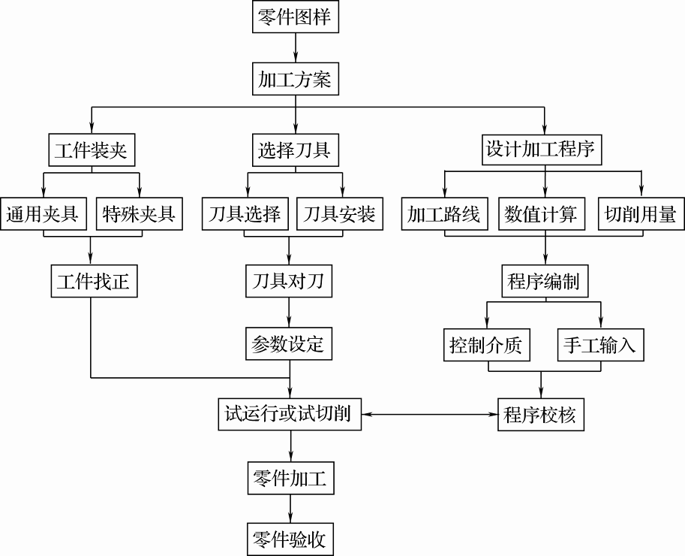
\includegraphics[width= \linewidth]{image/1-21}
		%    	\caption{}
		\label{fig:1-21}
	\end{figure}
\end{columns}
\end{frame}
\section{数控机床的种类}
\begin{frame}{数控机床的种类}

按工艺用途分类

A、金属切削类数控机床——数控车床、数控铣床、数控磨床、数控镗床以及加工中心。

B、金属成型类数控机床——数控折弯机、数控组合冲床、数控弯管机、数控回转头压力机等。这类机床起步晚,但目前发展很快。

C、数控特种加工机床——数控线切割机床、数控电火花机床、数控火焰切割机床、数控激光切割机床等。

D、其它类型数机床——数控三坐标测量机等。

\end{frame}

\begin{frame}{数控机床的种类}

按运动方式分类

A、点位控制数控机床——刀具点到点

B、直线控制数控机床——刀具平行于某一坐标轴移动

C、轮廓控制数控机床——刀具沿两个或两个以上的坐标轴同时移动。

\end{frame}

\begin{frame}{数控机床的种类}

按控制方式分类

A、开环控制系统

B、半闭环控制系统

C、闭环数控系统

\end{frame}

\begin{frame}{数控机床的种类}

按数控系统功能水平分类

数控机床按数控系统的功能水平可分为低、中、高三档。不同时期其划分标准也不同:

分辨率和进给速度

伺服进给类型

联运轴数

通信能力

显示功能

内装PLC

主CPU

高速、高效、高精度、高可靠性

模块化、智能化、柔性化和集成化

\end{frame}

\section{数控机床的坐标系}
\begin{frame}{数控机床的坐标系}
\begin{columns}
	\column{.4\textwidth}
	\begin{enumerate}
		\item 机床坐标系的定义
		\item 机床坐标系的规定 
		\item 机床坐标系的方向
	\end{enumerate} 
	\column{.6\textwidth}
	\begin{figure}
		\centering
		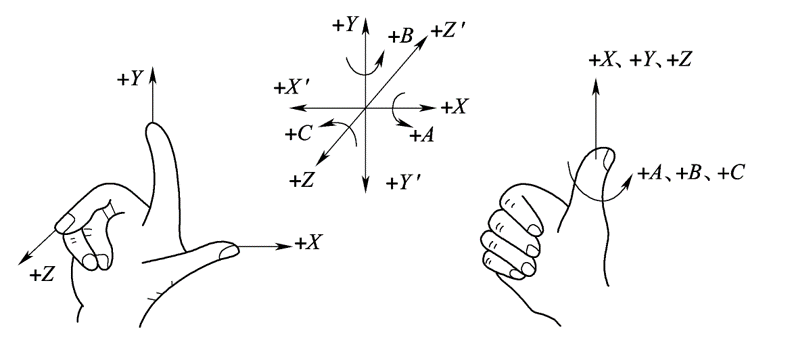
\includegraphics[width= \linewidth]{image/1-22}
		%    	\caption{}
		\label{fig:1-22}
	\end{figure}
\end{columns}
\end{frame}

\begin{frame}{数控机床的坐标系}
\begin{columns}
	\column{.3\textwidth}
	\begin{enumerate}
		\item Z轴方向
		\item X轴方向 
		\item Y轴方向
		\item 旋转轴方向
	\end{enumerate} 
	\column{.7\textwidth}
	\begin{figure}
		\centering
		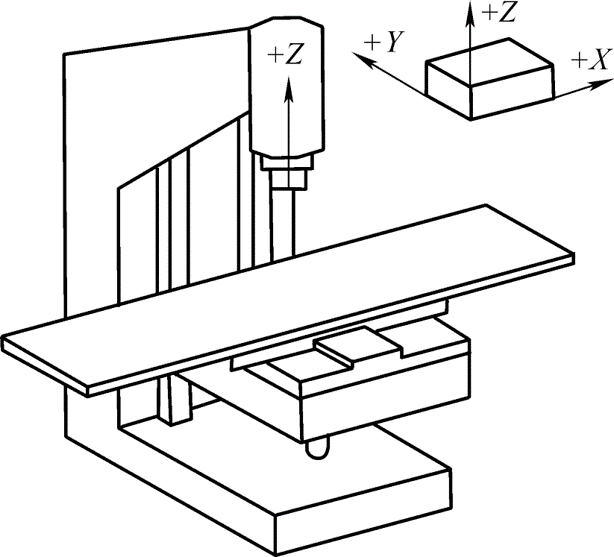
\includegraphics[width= 0.5\linewidth]{image/1-23}
		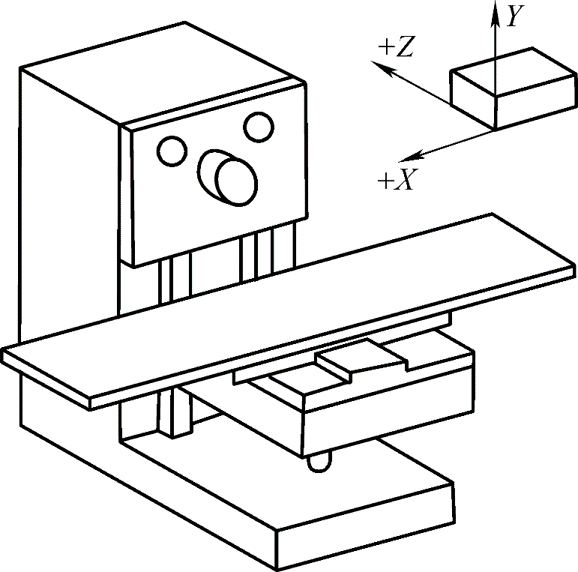
\includegraphics[width= 0.5\linewidth]{image/1-24}
		%    	\caption{}
		\label{fig:1-24}
	\end{figure}
\end{columns}
\end{frame}




\begin{frame}{作业}
\begin{enumerate}
	\item 简述数控机床的组成部分?
	\item 简述数控机床的分类?
\end{enumerate}
\end{frame}

\begin{frame}[plain]
\vfill

\centering \huge 谢谢大家!

\vfill

\flushleft \footnotesize   
~~~QQ:32731964\\
~~~TEL:18974681118\\
%~~~课件下载:\\
%~~~https://github.com/gnixoag/myworks2017/tree/master/jiaoshichengzhang

\end{frame}

\end{document} 
